\documentclass[11pt]{article}

\usepackage{fontspec}      % Gói chính để dùng font hệ thống với LuaLaTeX
\usepackage[vietnamese]{babel} % Gói hỗ trợ ngôn ngữ, tự động ngắt dòng TV

\usepackage{graphicx}
\usepackage{amsmath, amssymb, amsfonts, bm}
\usepackage{xcolor}
\usepackage{hyperref}
\usepackage{pifont}
\newcommand{\xmark}{\ding{55}} % ❌
\newcommand{\cmark}{\ding{51}} % ✅
\usepackage{array} % cần thêm trong preamble nếu chưa có
\usepackage{float}

\hypersetup{
    colorlinks=true,
    linkcolor=blue,
    filecolor=magenta,
    urlcolor=red,
    pdftitle={Overleaf Example},
    pdfpagemode=FullScreen,
}

\setmainfont{Times New Roman}
\setsansfont{Arial}
\setmonofont{Courier New}


% Page layout
\setlength{\topmargin}{-.5in}
\setlength{\textheight}{9.25in}
\setlength{\oddsidemargin}{0in}
\setlength{\textwidth}{6.8in}

% Title formatting
\usepackage{titling}
\setlength{\droptitle}{-10em}
\pretitle{%
	\begin{center}
	\LARGE\bfseries\textcolor{green} % Dòng tiêu đề đầu
	\end{center}
}
\posttitle{%
	\begin{center}
	\LARGE\bfseries\textcolor{cyan}  % Dòng tiêu đề thứ hai
	\end{center}
}
\title{{Module Project}\\[0.5em]\textcolor{cyan}{RAG (Retrieval-Augmented Generation) sử dụng Streamlit}}
\author{Đinh Nhật Thành}
\date{}
\renewcommand{\maketitle}{} % Ẩn tiêu đề mặc định

% Fancy header/footer
\usepackage{fancyhdr}
\pagestyle{fancy}
\fancyhf{}
\renewcommand{\footrulewidth}{0.4pt}
\lhead{\bfseries AI VIETNAM}
\rhead{\bfseries aivietnam.edu.vn}
\fancyfoot[C]{\thepage}

% Section format (không đánh số section)
\usepackage{titlesec}
\titleformat{\section}
{\normalfont\Large\bfseries}
{}{0em}{}

% Listings (code block)
\usepackage{listings}
\definecolor{codegreen}{rgb}{0,0.6,0}
\definecolor{codegray}{rgb}{0.5,0.5,0.5}
\definecolor{codepurple}{rgb}{0.58,0,0.82}
\definecolor{backcolour}{rgb}{0.95,0.95,0.92}
\lstdefinestyle{mystyle}{
    backgroundcolor=\color{backcolour},
    commentstyle=\color{codegreen},
    keywordstyle=\color{magenta},
    numberstyle=\tiny\color{codegray},
    stringstyle=\color{codepurple},
    basicstyle=\ttfamily\footnotesize,
    breaklines=true,
    captionpos=b,
    keepspaces=true,
    numbers=left,
    numbersep=5pt,
    tabsize=2,
    showspaces=false,
    showstringspaces=false,
    showtabs=false
}
\lstset{style=mystyle}

% Colored boxes
\usepackage[many]{tcolorbox}
\definecolor{sub}{HTML}{cde4ff}
\newtcolorbox{boxC}{
    colback = sub,
    boxrule = 0pt
}

% For math proofs or custom counters (tuỳ chọn nếu cần)
\usepackage{lipsum}
\newcounter{mycounter}
\newcommand\showmycounter{\stepcounter{mycounter}\themycounter}
\newcommand\showlips{\stepcounter{mycounter}\lipsum[\value{mycounter}]}

% Others
\usepackage{booktabs}
\usepackage{subcaption}
\usepackage{framed}
\usepackage{tikz}


%%%%%%%%%%%%%%%%%%%%%%%%%%%%%%%%%%%%%%%%%%%%%%%%%%%%%%%%%%%%%%%%%%%%%%%%%%%%%
%%%%%%%%%%%%%%%%%%%%%%%%%%%%%%%%%%%%%%%%%%%%%%%%%%%%%%%%%%%%%%%%%%%%%%%%%%%%%
%%%%%%%%%%%%%%%%%%%%%%%%%%%%%%%%%%%%%%%%%%%%%%%%%%%%%%%%%%%%%%%%%%%%%%%%%%%%%
\begin{document}
\maketitle

\begin{titlepage}
    \centering
    \vspace*{\fill}

    {\Huge \textbf{\thetitle} \par}
    \vspace{2em}

    {\Large \textbf{\theauthor} \par}
    \vspace{1em}

    {\large \today \par}

    \vspace*{\fill}
    \thispagestyle{fancy}
\end{titlepage}

\newpage
\tableofcontents
\thispagestyle{fancy}


%1%%%%%%%%%%%%%%%%%%%%%%%%%%%%%%%%%%%%%%%%%%%%%%%%%%%%%%%%%%%%%%%%%%%%%%%%%%%%%%%%%%%%%%%%%%%%%%%%%%%%%%%%%%%%%%%%%%%%%%%%%%%%%%%%%%%%%%%%%%%%%%%%%%%%%%%%%%%%%%%%%%%%%%%%%%%%%%%%%%%%%%%
\newpage

\renewcommand{\thesubsection}{\arabic{subsection}}
\newpage


\section{Tóm tắt ý chính}

Hệ thống được xây dựng nhằm hỗ trợ người dùng truy vấn thông tin từ tài liệu PDF bằng cách sử dụng mô hình ngôn ngữ lớn (LLM) kết hợp với cơ sở dữ liệu vector. Người dùng upload tài liệu PDF lên giao diện web được xây dựng bằng Streamlit, hệ thống sẽ tự động chia nhỏ văn bản, mã hoá thành vector, và sử dụng RAG để sinh ra câu trả lời theo truy vấn.

\section{Hệ thống RAG sử dụng Streamlit}

\subsection*{Kiến trúc hệ thống}

Hệ thống bao gồm các thành phần chính sau:

\begin{enumerate}
    \item Giao diện người dùng bằng \textbf{Streamlit}.
    \item Phân tích và trích xuất văn bản từ file PDF.
    \item Chia nhỏ nội dung thành các đoạn (chunk) bằng \texttt{SemanticChunker}.
    \item Mã hóa và lưu trữ các đoạn văn bản dưới dạng vector sử dụng \texttt{HuggingFaceEmbeddings} và cơ sở dữ liệu \texttt{Chroma}.
    \item Truy hồi thông tin liên quan dựa trên câu hỏi người dùng.
    \item Tạo prompt tùy chỉnh và gửi đến mô hình LLM để sinh câu trả lời.
\end{enumerate}

\begin{figure}[H]
    \centering
    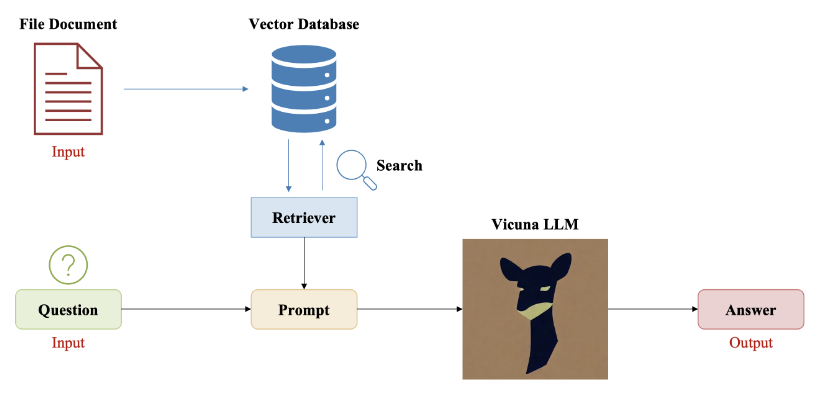
\includegraphics[width=0.85\textwidth]{architecture.png}
    \caption{Kiến trúc tổng quan của hệ thống RAG}
\end{figure}

\begin{lstlisting}[language=Python]
embeddings = HuggingFaceEmbeddings(
    model_name='bkai-foundation-models/vietnamese-bi-encoder')

model = AutoModelForCausalLM.from_pretrained("lmsys/vicuna-7b-v1.5", ...)
tokenizer = AutoTokenizer.from_pretrained("lmsys/vicuna-7b-v1.5")
pipeline = pipeline('text-generation', model=model, tokenizer=tokenizer)
\end{lstlisting}

\begin{lstlisting}[language=Python]
	embeddings = HuggingFaceEmbeddings(model_name='bkai-foundation-models/vietnamese-bi-encoder')
	loader = PyPDFLoader(tmp_file_path)
	documents = loader.load()

	splitter = SemanticChunker(embeddings=embeddings, ...)
	docs = splitter.split_documents(documents)
\end{lstlisting}


\begin{verbatim}
	loader = PyPDFLoader(tmp_file_path)
	vector_db = Chroma.from_documents(docs, embedding=embeddings)
	retriever = vector_db.as_retriever()
\end{verbatim}

\subsection*{3. Truy hồi văn bản liên quan}
\begin{verbatim}
st.set_page_config(page_title="PDF RAG Assistant")
uploaded_file = st.file_uploader("Tải PDF")
question = st.text_input("Đặt câu hỏi:")
\end{verbatim}

\subsection*{4. Giao diện Streamlit}

\begin{verbatim}
st.set_page_config(page_title="PDF RAG Assistant")
uploaded_file = st.file_uploader("Tải PDF")
question = st.text_input("Đặt câu hỏi:")
\end{verbatim}

\section{Prompting}

\subsection*{Mục tiêu prompt}
Prompt được thiết kế để đảm bảo mô hình trả về kết quả như mong đợi:

\subsection*{Prompt Thông Thường}

\subsection*{Prompt có chỉ dẫn, ví dụ}
\begin{verbatim}
Dựa vào nội dung sau, hãy:
1. Tóm tắt tối đa 3 ý chính, kèm theo số trang nếu có.
2. Trả lời câu hỏi bằng tiếng Việt ngắn gọn và chính xác.
3. Nếu không có thông tin liên quan, hãy để "answer" là "Không có dữ liệu liên quan".

Trả kết quả ở định dạng JSON như sau:

{
    "main_ideas": [
    {"point": "Ý chính 1", "source": "Trang ..."},
    {"point": "Ý chính 2", "source": "Trang ..."}
    ],
    "answer": "Câu trả lời"
}

Nội dung tài liệu: {context}
Câu hỏi: {question}
\end{verbatim}


\begin{verbatim}
Output:
	Nội
	Câu hỏi:
	Các mối đe dọa tầng cảm biến trong IoT

	Trả lời:
    * Khai thác thiết bị vật lý: Người tấn công có thể trích xuất dữ liệu từ bộ nhớ flash, trích xuất firmware, chiếm quyền shell root hoặc thậm chí cài đặt firmware có chứa mã độc. \\
    * Tấn công side-channel: Người tấn công có thể chiết xuất khóa bí mật dùng để mã hóa/giải mã hoặc trộm cắp dữ liệu nhạy cảm bên trong. \\
    * Chỉnh sửa firmware: Người tấn công có thể lợi dụng việc thiếu cơ chế xác thực chặt chẽ trong quá trình cập nhật firmware qua OTA. \\

\end{verbatim}

\end{document}